\documentclass[conference]{IEEEtran}
\IEEEoverridecommandlockouts
% The preceding line is only needed to identify funding in the first footnote. If that is unneeded, please comment it out.
\usepackage{cite}
\usepackage{amsmath,amssymb,amsfonts}
\usepackage{algorithmic}
\usepackage{graphicx}
\usepackage{textcomp}
\usepackage{xcolor}
\usepackage{hyperref}
\usepackage{caption}
\def\BibTeX{{\rm B\kern-.05em{\sc i\kern-.025em b}\kern-.08em
    T\kern-.1667em\lower.7ex\hbox{E}\kern-.125emX}}
\begin{document}

\title{Deep Learning for Distinguish AI Generated Images\\
}

\author{\IEEEauthorblockN{Chuxuan Yin}
\IEEEauthorblockA{\textit{Rice University} \\
6100 Main St, Houston, TX 77005 \\
cy48@rice.edu}
}

\maketitle

\begin{abstract}
AI painting is an emerging field. Although there is some controversy over how to use it,
it is without a doubt one of the most successful applications of generative models in industrial production.
How to distinguish whether a image is generated by AI is a topic that is always concerned by people, while it is
not fully developed yet. In this paper, we will try to categorize this problem as an image style recognition problem,
and use some well-developed models to classify AI generated images. Specifically, we will train ResNet50, fine-tuning
GoogleNet and ViT on different kinds of dataset, and compared their performance based on some benchmark. Then we'll combine
all the different kinds of images into one dataset and try to train models on it. We'll test our model in this way in order
to see whether our model could capture some common features among different categories of AI generated images. The result of
our experiments show that current image classification model could really distinguish AI generated images to a certain degree.
\end{abstract}

\section{Introduction}
In the last mouths, AI painting suddenly began to attract people's attention. With the implementation of the stable diffusion framework, AI painting
finally showed its great potential on large scale commercial usages. People who know nothing about painting could also easily use this model to generate
high quality images in just one minute. While AI painting looked really awesome, it also raised some critques, one of these is that those generated images are
very homogenized, so they are unable to substitue the hand-writting pictures. Although this is a very controversial topic, we could try to think this problem in
a different way: do AI generated images really have some features in common? While it might be a hard task for human eyes to distinguish these slight differences,
AI itself could be a good classifier. In fact, if we think of AI-generated images as images of a certain style, then this problem is really close to the fine-grained
image classification problem which we are familiar with. With the inspiration of this idea, we'll conduct a fine-grained image classification way to solve this problem in this paper.

According to the literature review[1], we know that there are four mainstream methods for fine-grained image classification based on deep learning:
\begin{itemize}
    \item The first one is based on regular image classification model such as AlexNet, ResNet[2], GoogleNet, etc. Although these models have strong representational capabilities, their performace on fine-grained classification is not very ideal. The common solution is using some pre-trained weights trained on ImageNet, then fine-tune this model to get a final result.    
    \item The second one is the fine-grained feature learning method. In the paper [3] published in ICCV in 2015, Lin et al. proposed a bilinear convolutional neural network model to achieve a better representation of deep convolutional features. This method uses two networks, VGG-D and VGG-M, as the benchmark network. Without using the Bounding Box (border) label information, it reaches a classification accuracy of 84.1\% on the CUB200-2011 dataset; while using the Bounding Box, its classification accuracy is as high as 85.1.
    \item The third one is object part based detection. The idea of the method based on object part detection is: first detect the position of the target in the image, and then detect the position of the discriminative area in the target, and then combine the target image and the discriminative area the target region blocks are simultaneously fed into a deep convolutional network for classification. One of the representative work is the Part-RCNN method proposed in 2014 ECCV[4].
    \item The last one is vision attention method. This method is inspired by the vision attention mechanism in human beings, and is widely adopted in computer vision afterwards. Since vision attention model could identify discriminative area in images without labels, it showed a great potential in fine-grained image classification. The recurrent attention convolutional neural network proposed in the 17-year CVPR is a representative work[5].
\end{itemize}

\section{Dataset}

Since this is a totally new field, we do not have off-the-shelf dataset, so we need to count on ourselves to collect data. Basically we need two different kinds of images: AI-generated images and
hand-drawing images. The former can be generated with models, and the latter could be found on website. But there is a key issue: we need to make sure that AI-generated images and hand-drawing images
are basically looked the same for human beings, so that our experiment result would not be affected by other factors.

On the basis of above, we decide to collect three specific genres of images: the avatar of Ganyu(a game character) in manga style, the castle in fantasy tyle, and the sports car in realistic style.
We collect 200 training and 100 testing images for these three different kinds of images separately. And we also mixed these images up to make a big dataset to test the generalizability of the model.
For each image, we preprocessed it to fit 200 * 200 dimension.

\begin{center}
  \begin{minipage}{0.24\textwidth}
    \centering
      \begin{minipage}{.5\textwidth}
        \centering
        
\includegraphics[width=0.9\linewidth]{ganyu1.jpg}
        \label{fig:test1}
      \end{minipage}%
      \begin{minipage}{.5\textwidth}
        \centering
        
\includegraphics[width=0.9\linewidth]{ganyu2.jpg}
        \label{fig:test2}
    \end{minipage}
    \captionof{figure}{Avatar}
  \end{minipage}
  \begin{minipage}{0.24\textwidth}
    \centering
      \begin{minipage}{.5\textwidth}
        \centering
        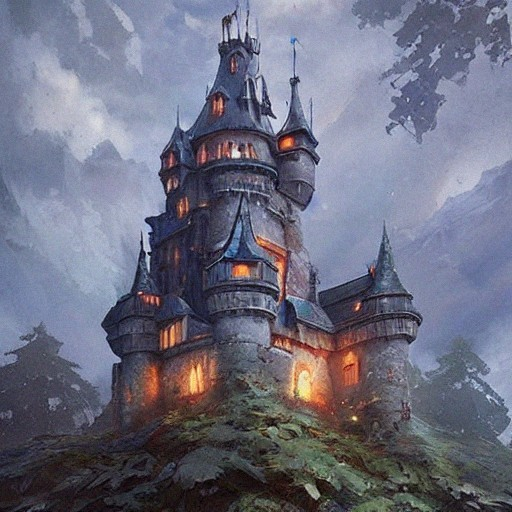
\includegraphics[width=0.9\linewidth]{castle1.jpg}
        \label{fig:test1}
      \end{minipage}%
      \begin{minipage}{.5\textwidth}
        \centering
        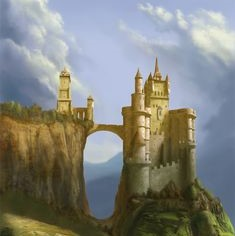
\includegraphics[width=0.9\linewidth]{castle2.jpg}
        \label{fig:test2}
    \end{minipage}
    \captionof{figure}{Castle}
  \end{minipage}
  \begin{minipage}{0.24\textwidth}
    \centering
      \begin{minipage}{.5\textwidth}
        \centering
        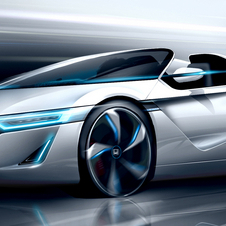
\includegraphics[width=0.9\linewidth]{sports_car1.jpg}
        \label{fig:test1}
      \end{minipage}%
      \begin{minipage}{.5\textwidth}
        \centering
        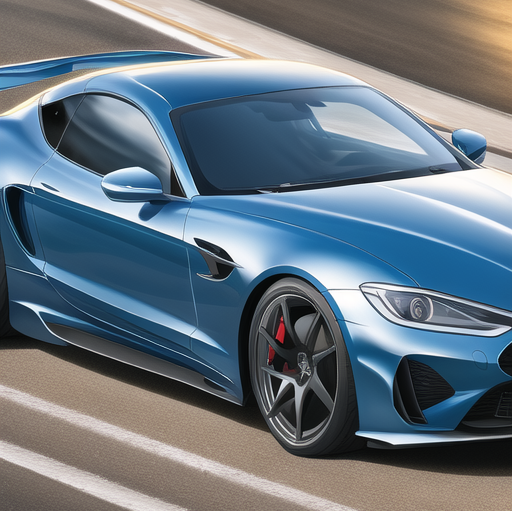
\includegraphics[width=0.9\linewidth]{sports_car2.jpg}
        \label{fig:test2}
    \end{minipage}
    \captionof{figure}{Sports car}
  \end{minipage}
\end{center}

\section{Models}

We'll use three different kinds of models to test our dataset: ResNet50, GoogleNet and ViT. The reason why we choose these three models is that they are all very popular and widely used in image classification. We'll use the same training and testing dataset for all the models, and compare their performance based on the accuracy of the model.

\subsection{ResNet50}
A resisual network is a deep neural network that is trained with residual learning. The residual learning framework eliminates the vanishing gradient problem, and improves the accuracy and speed of training. The ResNet50 is a 50-layer residual network, which is the most popular one in the field of image classification. ResNet50 is also widely
used in fine-grained image classification. We use the ResNet50 model provided by PyTorch to train our dataset. Instead of using given pre-trained weights that trained on ImageNet, we train the model from scratch. The reason why we do not use pre-trained weights is that we want to make sure that the model is not affected by those irrelevent
images in ImageNet.

\begin{figure}[h]
\centering
  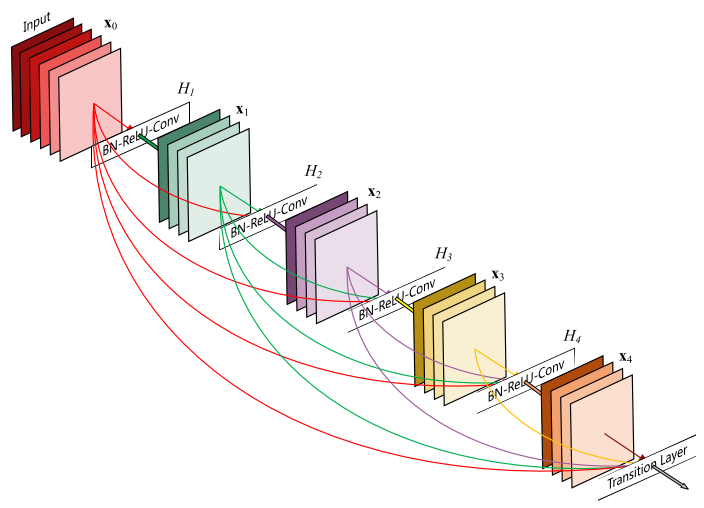
\includegraphics[width=0.6\linewidth]{resnet_model.png}
\caption{ResNet model}
\end{figure}

\subsection{GoogleNet}

GoogleNet is a efficient convolutional neural network in image classification which is 22 layers deep. One method the GoogLeNet achieves efficiency is through reduction of the input image, while simultaneously retaining important spatial information. Different from the way we train ResNet50, we choose to use its pre-trained weights that trained on ImageNet,
then fine-tune the model on our dataset. We do this because using fine-tuning model is a very useful technique in fine-grained image classification even if consider the affect of images. Here we do a control experiment to see if the pre-trained weights would affect the performance of the model.

\begin{figure}[h]
\centering
  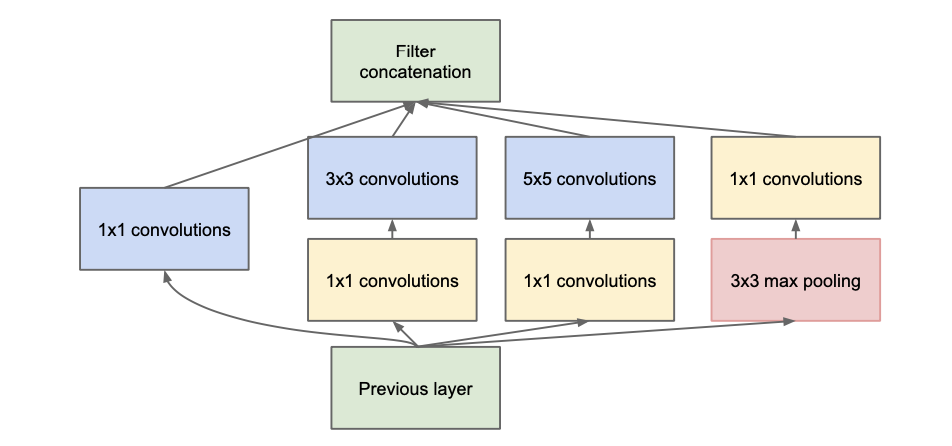
\includegraphics[width=0.8\linewidth]{googlenet_model.png}
\caption{GoogleNet model}
\end{figure}

\subsection{ViT}

Visual attention mechanism is another popular technique in fine-grained image classification. Attention mechanism gives the nerual network the possibility to see the tiny difference between different images in same category. The ViT is a visual model based on the architecture of a transformer originally designed for text-based tasks, while the computational
resources for pre-training is less than CNN. The model also learns on training data to encode the relative location of the image patches to reconstruct the structure of the image. We also train ViT model on our dataset from scratch. The reason is the same for training ResNet50.

\begin{figure}[h]
\centering
  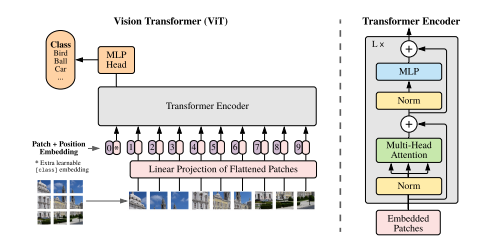
\includegraphics[width=0.8\linewidth]{ViT_model.png}
\caption{ViT model}
\end{figure}

\section{Experiments and Results}

Due to the limitation of time and computing resources, we only train the model for 300 epochs. This is enough for us to show the tendency of convergence and get a clear understanding of the ability for each model to classify our dataset. For other hyperparameters, we choose to train models in batch-size 100 to control the stability of our training process.
We also use SGD optimizer with learning rate 1e-3 to improve the training efficiency. Finally we use cross entropy loss function for this classification problem.

\subsection{Training on Dataset of Single Image Category}

First we'll look at the performace of ResNet50. Here we display the training loss and accuracy of each model on avatar dataset. From the training loss and accuracy curve we can see that the loss function does not convege very well during the training process. But we can see the tendency that the training loss is decreasing and the accuracy is increasing. The test accuracy of
trained ResNet50 model is around 0.7, which means after training, ResNet50 could really identify the AI generated avatar images to a certain degree, but the trembling curve indicates that this model doesn't fit our dataset very well.

\begin{figure}[h]
  \centering
    \begin{minipage}{.24\textwidth}
      \centering
      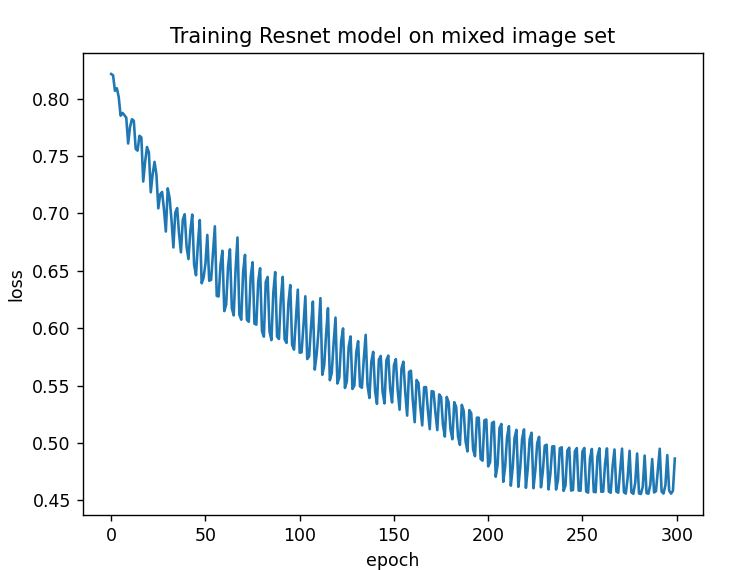
\includegraphics[width=0.9\linewidth]{resnet_ganyu_loss.jpg}
      \label{fig:test1}
    \end{minipage}%
    \begin{minipage}{.24\textwidth}
      \centering
      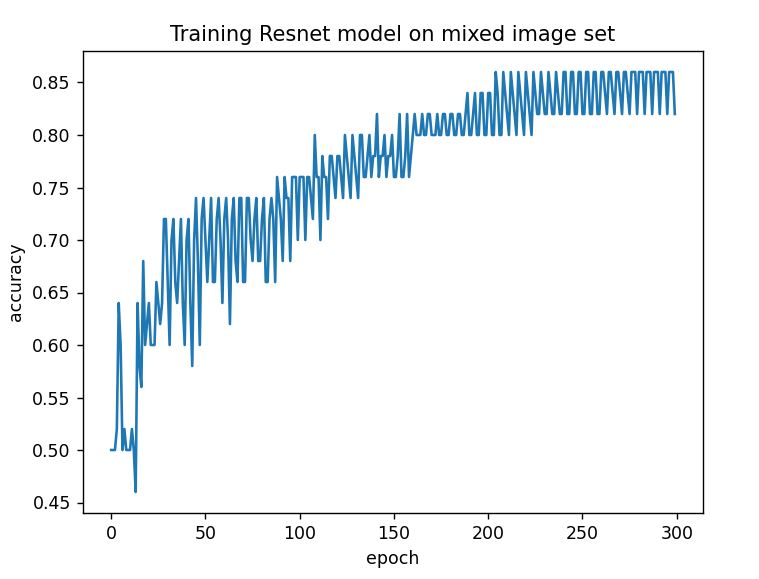
\includegraphics[width=0.9\linewidth]{resnet_ganyu_accuracy.jpg}
      \label{fig:test2}
    \end{minipage}
  \captionof{figure}{training performance on avatar dataset for ResNet50}
\end{figure}

Then we try to train GoogleNet on the same dataset. As we described before, we load the GoogLeNet model with the pre-trained weights on ImageNet, and start to train it on our own dataset. We can see that for the single category image dataset, GoogLeNet model achieved great performance. It's loss function is much more smooth than ResNet50 and it converges very fast. The test
accuracy of 0.8 also shows its ability of predicting the AI generated avatar images.

\begin{figure}[h]
  \centering
    \begin{minipage}{.24\textwidth}
      \centering
      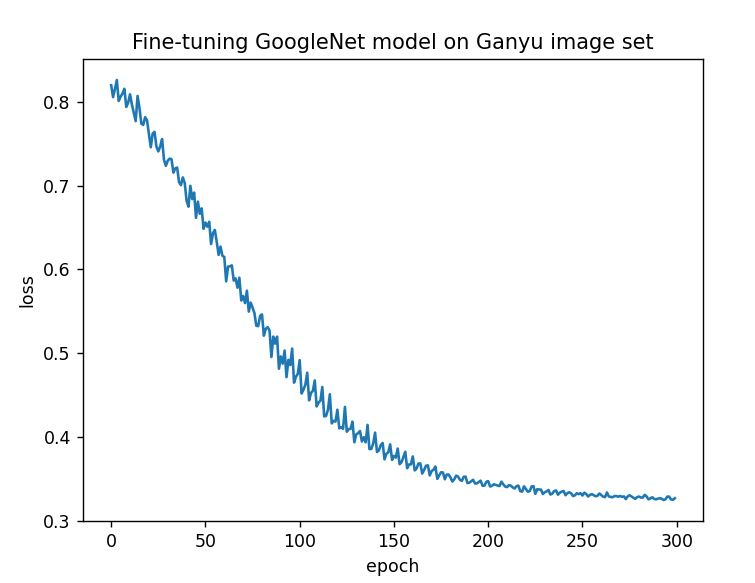
\includegraphics[width=0.9\linewidth]{googlenet_ganyu_loss.jpg}
      \label{fig:test1}
    \end{minipage}%
    \begin{minipage}{.24\textwidth}
      \centering
      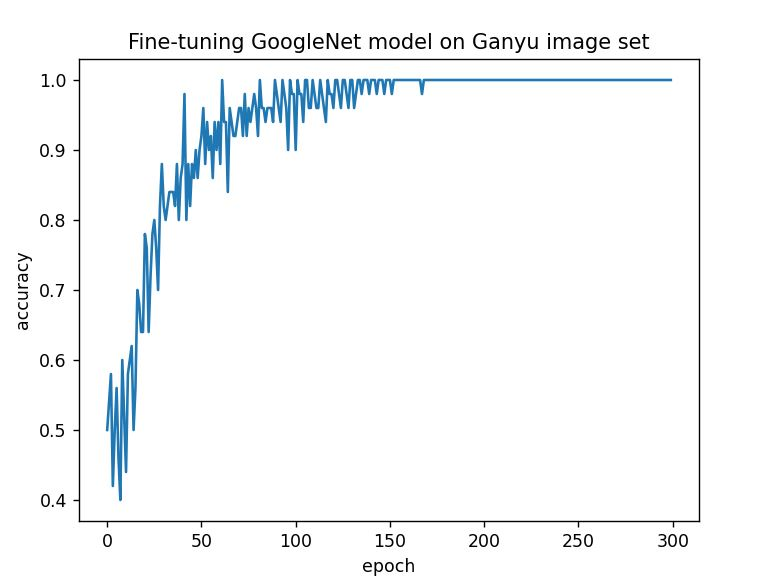
\includegraphics[width=0.9\linewidth]{googlenet_ganyu_accuracy.jpg}
      \label{fig:test2}
    \end{minipage}
  \captionof{figure}{training performance on avatar dataset for GoogleNet}
\end{figure}

Finally we turn to see the performance of ViT model. Unfortunately, the ViT model didn't perform well on our dataset. The loss function is not smooth and the accuracy is not increasing. The test accuracy is only 0.6, which means the model is not able to identify the AI generated avatar images.

\begin{figure}[h]
  \centering
    \begin{minipage}{.24\textwidth}
      \centering
      \includegraphics[width=0.9\linewidth]{ViT_ganyu_loss.jpg}
      \label{fig:test1}
    \end{minipage}%
    \begin{minipage}{.24\textwidth}
      \centering
      \includegraphics[width=0.9\linewidth]{ViT_ganyu_accuracy.jpg}
      \label{fig:test2}
    \end{minipage}
  \captionof{figure}{training performance on avatar dataset for ViT}
\end{figure}

From the above results, we can see that pre-trained weights do affect the performance of the model. The pre-trained GoogleNet fits very well on our dataset, which means the weight gained from other ImageNet helps a lot in identifying AI genrated images. While visual attention mechanism does not work
very well on our dataset, this might be explained as we can't recgonize the AI generated images by observing the local details.

\subsection{Training on Dataset of Multiple Image Categories}

After we train the model on single category image dataset, we try to train the model on the dataset with mixed images. This could show that whether our model could capture some common features of the AI generated images, or our model is just be trained to classify a certain type of images in the previous
experiments. Here are the training results of ResNet50, GoogleNet and ViT model on the mixed dataset.

\begin{figure}[h]
  \centering
    \begin{minipage}{.24\textwidth}
      \centering
      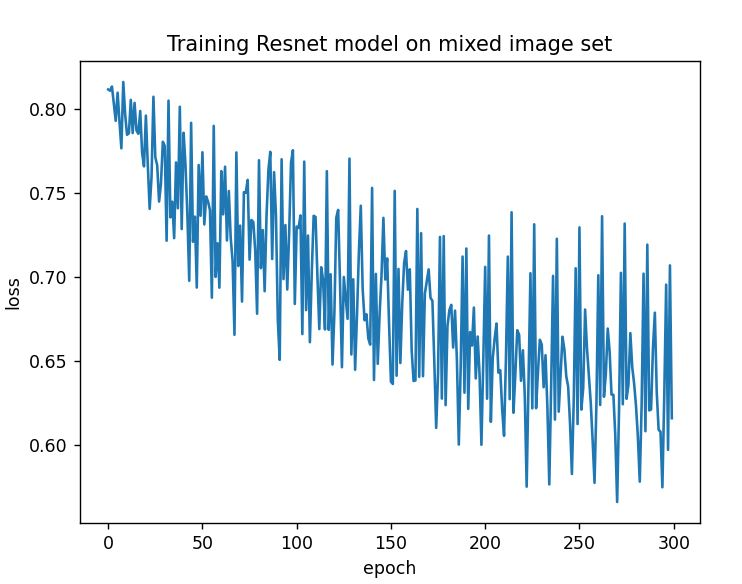
\includegraphics[width=0.9\linewidth]{resnet_mixed_loss.jpg}
      \label{fig:test1}
    \end{minipage}%
    \begin{minipage}{.24\textwidth}
      \centering
      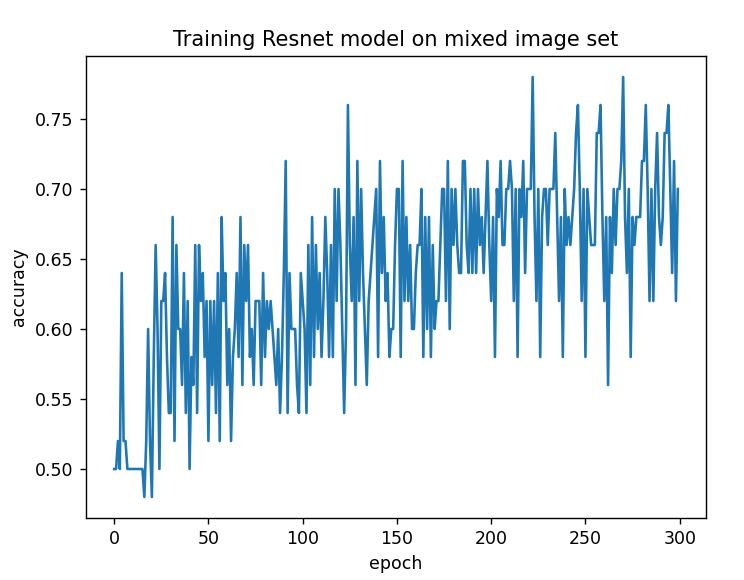
\includegraphics[width=0.9\linewidth]{resnet_mixed_accuracy.jpg}
      \label{fig:test2}
    \end{minipage}
  \captionof{figure}{training performance on mixed dataset for ResNet50}
\end{figure}

\begin{figure}[h]
  \centering
    \begin{minipage}{.24\textwidth}
      \centering
      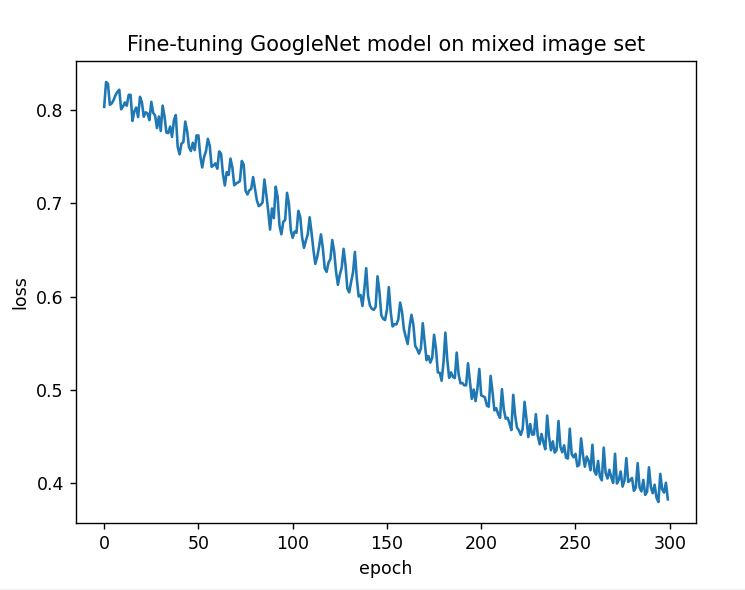
\includegraphics[width=0.9\linewidth]{googlenet_mixed_loss.jpg}
      \label{fig:test1}
    \end{minipage}%
    \begin{minipage}{.24\textwidth}
      \centering
      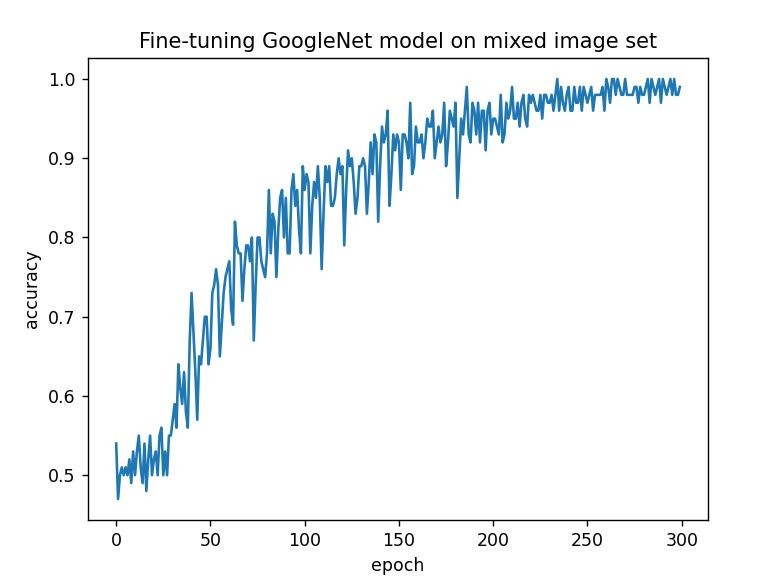
\includegraphics[width=0.9\linewidth]{googlenet_mixed_accuracy.jpg}
      \label{fig:test2}
    \end{minipage}
  \captionof{figure}{training performance on mixed dataset for GoogleNet}
\end{figure}

\begin{figure}[h]
  \centering
    \begin{minipage}{.24\textwidth}
      \centering
      \includegraphics[width=0.9\linewidth]{ViT_mixed_loss.jpg}
      \label{fig:test1}
    \end{minipage}%
    \begin{minipage}{.24\textwidth}
      \centering
      \includegraphics[width=0.9\linewidth]{ViT_mixed_accuracy.jpg}
      \label{fig:test2}
    \end{minipage}
  \captionof{figure}{training performance on mixed dataset for ViT}
\end{figure}

Unsurprisingly, our models performed much worse on the mixed dataset. ResNet50 and ViT model are not even converged after 300 epochs of training, and the loss function curve of fine-tuning GoogleNet also trembles a little bit more than the previous experiments. But even in this case, the fine-tuning GoogleNet still showed its great fitness of our dataset.
And the test accuracy achieved 0.7, which means our model gives its prediction based on some logic while not just throw a random try.

\section{Conclusion}

In this paper, we have explored the possibility of using mature fine-grained image classification model to identify AI generated images. We choosed three different kind models to train on the dataset of one category images and the dataset of mixed images. The results show that for current AI generated images, fine-tuning model could classify them with a relatively
high accuracy, and it could really caputres some internal features of AI-generated images to a certain degree. This result really help us understand more about AI painting, let us carefully review the difference and connection between AI painting and human painting, which may affect how we use AI painting in the future. 

\begin{thebibliography}{1}
  \bibitem{Xiushen Wei}
  Xiushen Wei, Yizhe Song, et al. Fine-Grained Image Analysis With Deep Learning: A Survey. \emph{IEEE Transactions on Pattern Analysis and Machine Intelligence }, Dec 2022.
  
  \bibitem{Kaiming}
  Kaiming He, Xiangyu Zhang, Shaoqing Ren, Jian Sun. Deep Residual Learning for Image Recognition. \emph{IEEE Conference on Computer Vision and Pattern Recognition}, June 2016.

  \bibitem{ZHANG}
  ZHANG, Xiaofan, et al. Embedding label structures for fine-grained feature representation. \emph{Proceedings of the IEEE Conference on Computer Vision and Pattern Recognition}, May 2016. 

  \bibitem{Zhang}
  Zhang N, Donahue J, Girshick R B, et al. Part-Based R-CNNs for Fine-Grained Category Detection. \emph{European Conference on Computer Vision}, Nov 2014

  \bibitem{Volodymyr}
  Volodymyr Mnih, Nicolas Heess, Alex Graves and KorayKavukcuoglu. Recurrent Models of Visual Attention. \emph{Advances in Neural Information Processing Systems}, June 2014.
\end{thebibliography}

\end{document}
